\input{../../templates/exercises_preamble.tex}

\usepackage[linguistics]{forest} %for syntax trees

\begin{document}

%Title
\def \sheetnr {09}
\def \sheettitle {Trees and X-bar theory}
\def \handedout {Monday 22\textsuperscript{nd} July, 14:00}
\def \tosubmit {Monday 29\textsuperscript{th} July, 14:00}
\def \totalpoints {8}
\setuptitle

%Ex 01
\begin{task}{Traversal}{2}
Implement a pre-order and a post-order traversal by filling in the bodies of the methods \texttt{Tree.preorder(self)} and \texttt{Tree.postorder(self)}. The methods should take a tree node as an argument and return a list of the nodes of the tree in the respective order (careful: not a list of the \emph{names} of the nodes, but a list of the node objects themselves, so you can later perform operations on the subtrees in the list. You can use the given function \texttt{names(nodelist)} to turn a list of tree nodes into a list of just the names of these nodes). You can take the existing implementation of \texttt{inorder(self)} as a reference, and use the given printout methods to have your tree objects nicely displayed during testing.\\

\textit{Examples:}\begin{lstlisting}{console}
########
# Defining a book tree object
########
# - Book
# - - Chapter 1
# - - - Section 1.1
# - - - Section 1.2
# - - Chapter 2
# - - - Section 2.1
# - - - - Subsection 2.1.1
# - - - - Subsection 2.1.2
# - - Chapter 3
> book = Tree('Book', [
    Tree('Chapter 1', [Tree('Section 1.1'), Tree('Section 1.2')]),
    Tree('Chapter 2', [Tree('Section 2.1',
        [Tree('Subsection 2.1.1'), Tree('Subsection 2.1.2')])]),
    Tree('Chapter 3')
    ])

########
# Printing out the tree object
########

> book.printout_oneline()
[Book [Chapter 1 [Section 1.1], [Section 1.2]], [Chapter 2 [Section 2.1 
[Subsection 2.1.1], [Subsection 2.1.2]]], [Chapter 3]]

> book.prinout_plain()
Book
   Chapter 1
      Section 1.1
      Section 1.2
   Chapter 2
      Section 2.1
         Subsection 2.1.1
         Subsection 2.1.2
   Chapter 3

> book.printout_fancy()
|--Book
   |--Chapter 1
   |  |--Section 1.1
   |  |--Section 1.2
   |  
   |--Chapter 2
   |  |--Section 2.1
   |     |--Subsection 2.1.1
   |     |--Subsection 2.1.2
   |  
   |--Chapter 3


########
# Preorder and postorder
########
> Tree.names(book.preorder())
['Book', 'Chapter 1', 'Section 1.1', 'Section 1.2', 'Chapter 2',
'Section 2.1', 'Subsection 2.1.1', 'Subsection 2.1.2', 'Chapter 3']
> Tree.names(book.postorder())
['Section 1.1', 'Section 1.2', 'Chapter 1', 'Subsection 2.1.1',
'Subsection 2.1.2', 'Section 2.1', 'Chapter 2', 'Chapter 3', 'Book']
\end{lstlisting}
%\textit{Examples:}\begin{lstlisting}{console}
%> abc = Tree('A', [
%            Tree('B', [Tree('D')]),
%            Tree('C', [Tree('E'), Tree('F'), Tree('G', [Tree('H')])])
%        ])
%> Tree.names(abc.preorder())
%['A', 'B', 'D', 'C', 'E', 'F', 'G', 'H']
%> Tree.names(abc.postorder())
%['D', 'B', 'E', 'F', 'H', 'G', 'C', 'A']
%\end{lstlisting}
\end{task}

%Ex 02
\begin{task}{X-bar check}{6}
Before approaching this task, please read up on the theoretical background in \texttt{theory\_ex\_09.pdf}.\\

Write method \texttt{Tree.is\_xbar(self)} that, given a tree object as an input, returns \texttt{True} or \texttt{False} depending on whether or not the tree is in accordance with the rules of X-bar theory. To do so, fill in the missing bodies in the sections commented "\texttt{check projection levels}" (you can take the given implementation of \texttt{Tree.is\_phrase\_projection(self)} as an example on how to write the other methods in the block) and "\texttt{check structural constraints}" (you can take the given implementation of \texttt{Tree.is\_complement\_structure(self)} as an example on how to write the other methods in the block).\\

\textit{Examples:}\begin{lstlisting}{console}
#########
# Definitions of some tree objects to play around with
#########
> cat_terminal = Tree('cat')
> cat_N = Tree('N0', [cat_terminal])
> cat_Nbar = Tree('N1', [cat_N])
> cat_NP = Tree('N2', [cat_Nbar])

> the = Tree('D2', [Tree('D1', [Tree('D0', [Tree('the')])])])
> the_cat = Tree('N2', [the, cat_Nbar])
> small = Tree('A2', [Tree('A1', [Tree('A0', [Tree('small)]])])])
> small_cat = Tree('N1', [small, cat_Nbar])
> on_the_mat = Tree('P2', [Tree('P1',
    [Tree('P0', [Tree('on')]),
    Tree('N2',
        [Tree('D2', [Tree('D1', [Tree('D0', [Tree('the')])])]),
        Tree('N1', [Tree('N0', [Tree('mat')])])])
    ])])

> cat_wrong_category_mismatch = Tree('P2', [the, Tree('N1', [cat_N])])
> cat_wrong_two_heads = Tree('N1', [cat_N, cat_N])

#########
# Some tests for projection levels
#########
> the_cat.is_xbar()
True
> small_cat.is_xbar()
True
> cat_wrong_category_mismatch.is_xbar()
False  # because categories of phrase and bar don't match,
# so it's not a proper phrase, so not a proper x-bar structure

> cat_N.is_head_projection()
True
> cat_Nbar.is_bar_projection()
True
> cat_NP.is_phrase_projection()
True
> cat_NP.is_bar_proection()
False  # because it is a phrase, not a bar projection
> cat_wrong_category_mismatch.is_xbar()
False  # see above

#########
# Some tests for structural constraints
#########
> the_cat.is_no_specifer_structure()
False  # because it doesn't branch unary into just bar,
# but binary with the speicfier "the"
> the_cat.is_specifer_structure()
True  # same argument

> small_cat.is_no_adjunct_or_complement_structure()
False  # because it has the adjunct "small"
> small_cat.is_adjunct_structure()
True  # because it has the adjunct "small"
> small_cat.is_complement_structure()
False  # because there is no complement
> on_the_mat.is_complement_structure()
True  # because it has the complement "the mat"

> cat_N.is_head_structure()
True
> cat_NP.is_head_structure()
False
> cat_wrong_to_heads.is_head_structure()
False  # because it doesn't branch unary into 1, but binary into 2 heads


\end{lstlisting}

\medskip

\textbf{Important}: One of the main purposes of this assignment is to practice \textit{recursion}. The well-formedness of a tree is a recursive concept, so it needs to be recursively verified. For example, in the second illustration of an ill-formed tree in the theory file, the ill-formedness is hidden inside a substructure: There is a category mismatch between DP and P', so the DP specifier is not well-formed, \textit{so the NP as a whole isn't either}. Although on the top-most level, the labels make it look like an NP branching into a specifier and a bar projection is in accordance with the rules of X-bar theory, the internal structure of the DP is flawed, and therefore the surrounding NP tree, which has the ill-formed DP as a subtree, does not qualify as a well-formed X-bar tree in whole. Your program must detect that. In the methods you write, you have to carry out recursive function calls on the tree and descend into the substructure of a tree. It does not suffice to just check the name of the labels on the top-most levels, because the labels might be lying; if your tree verification ends at the first level of children of the root node, it is wrong. W.r.t.\ the example given here, it does not suffice to check that the node labelled NP branches into something labeld DP and something labelled N'; instead, you have to check that the DP is indeed a well-formed phrase projection and that the N' is an actual bar projection by making recursive function calls on the child nodes of the NP. Verify the behavior of your functions using the tests provided, and try to understand why some of the structures are not in accordance with the rules of X-bar theory while others are.\\

To help you understand the way the functions interact with each other and where the recursion enters, here is an illustration of the call hierarchy:\\
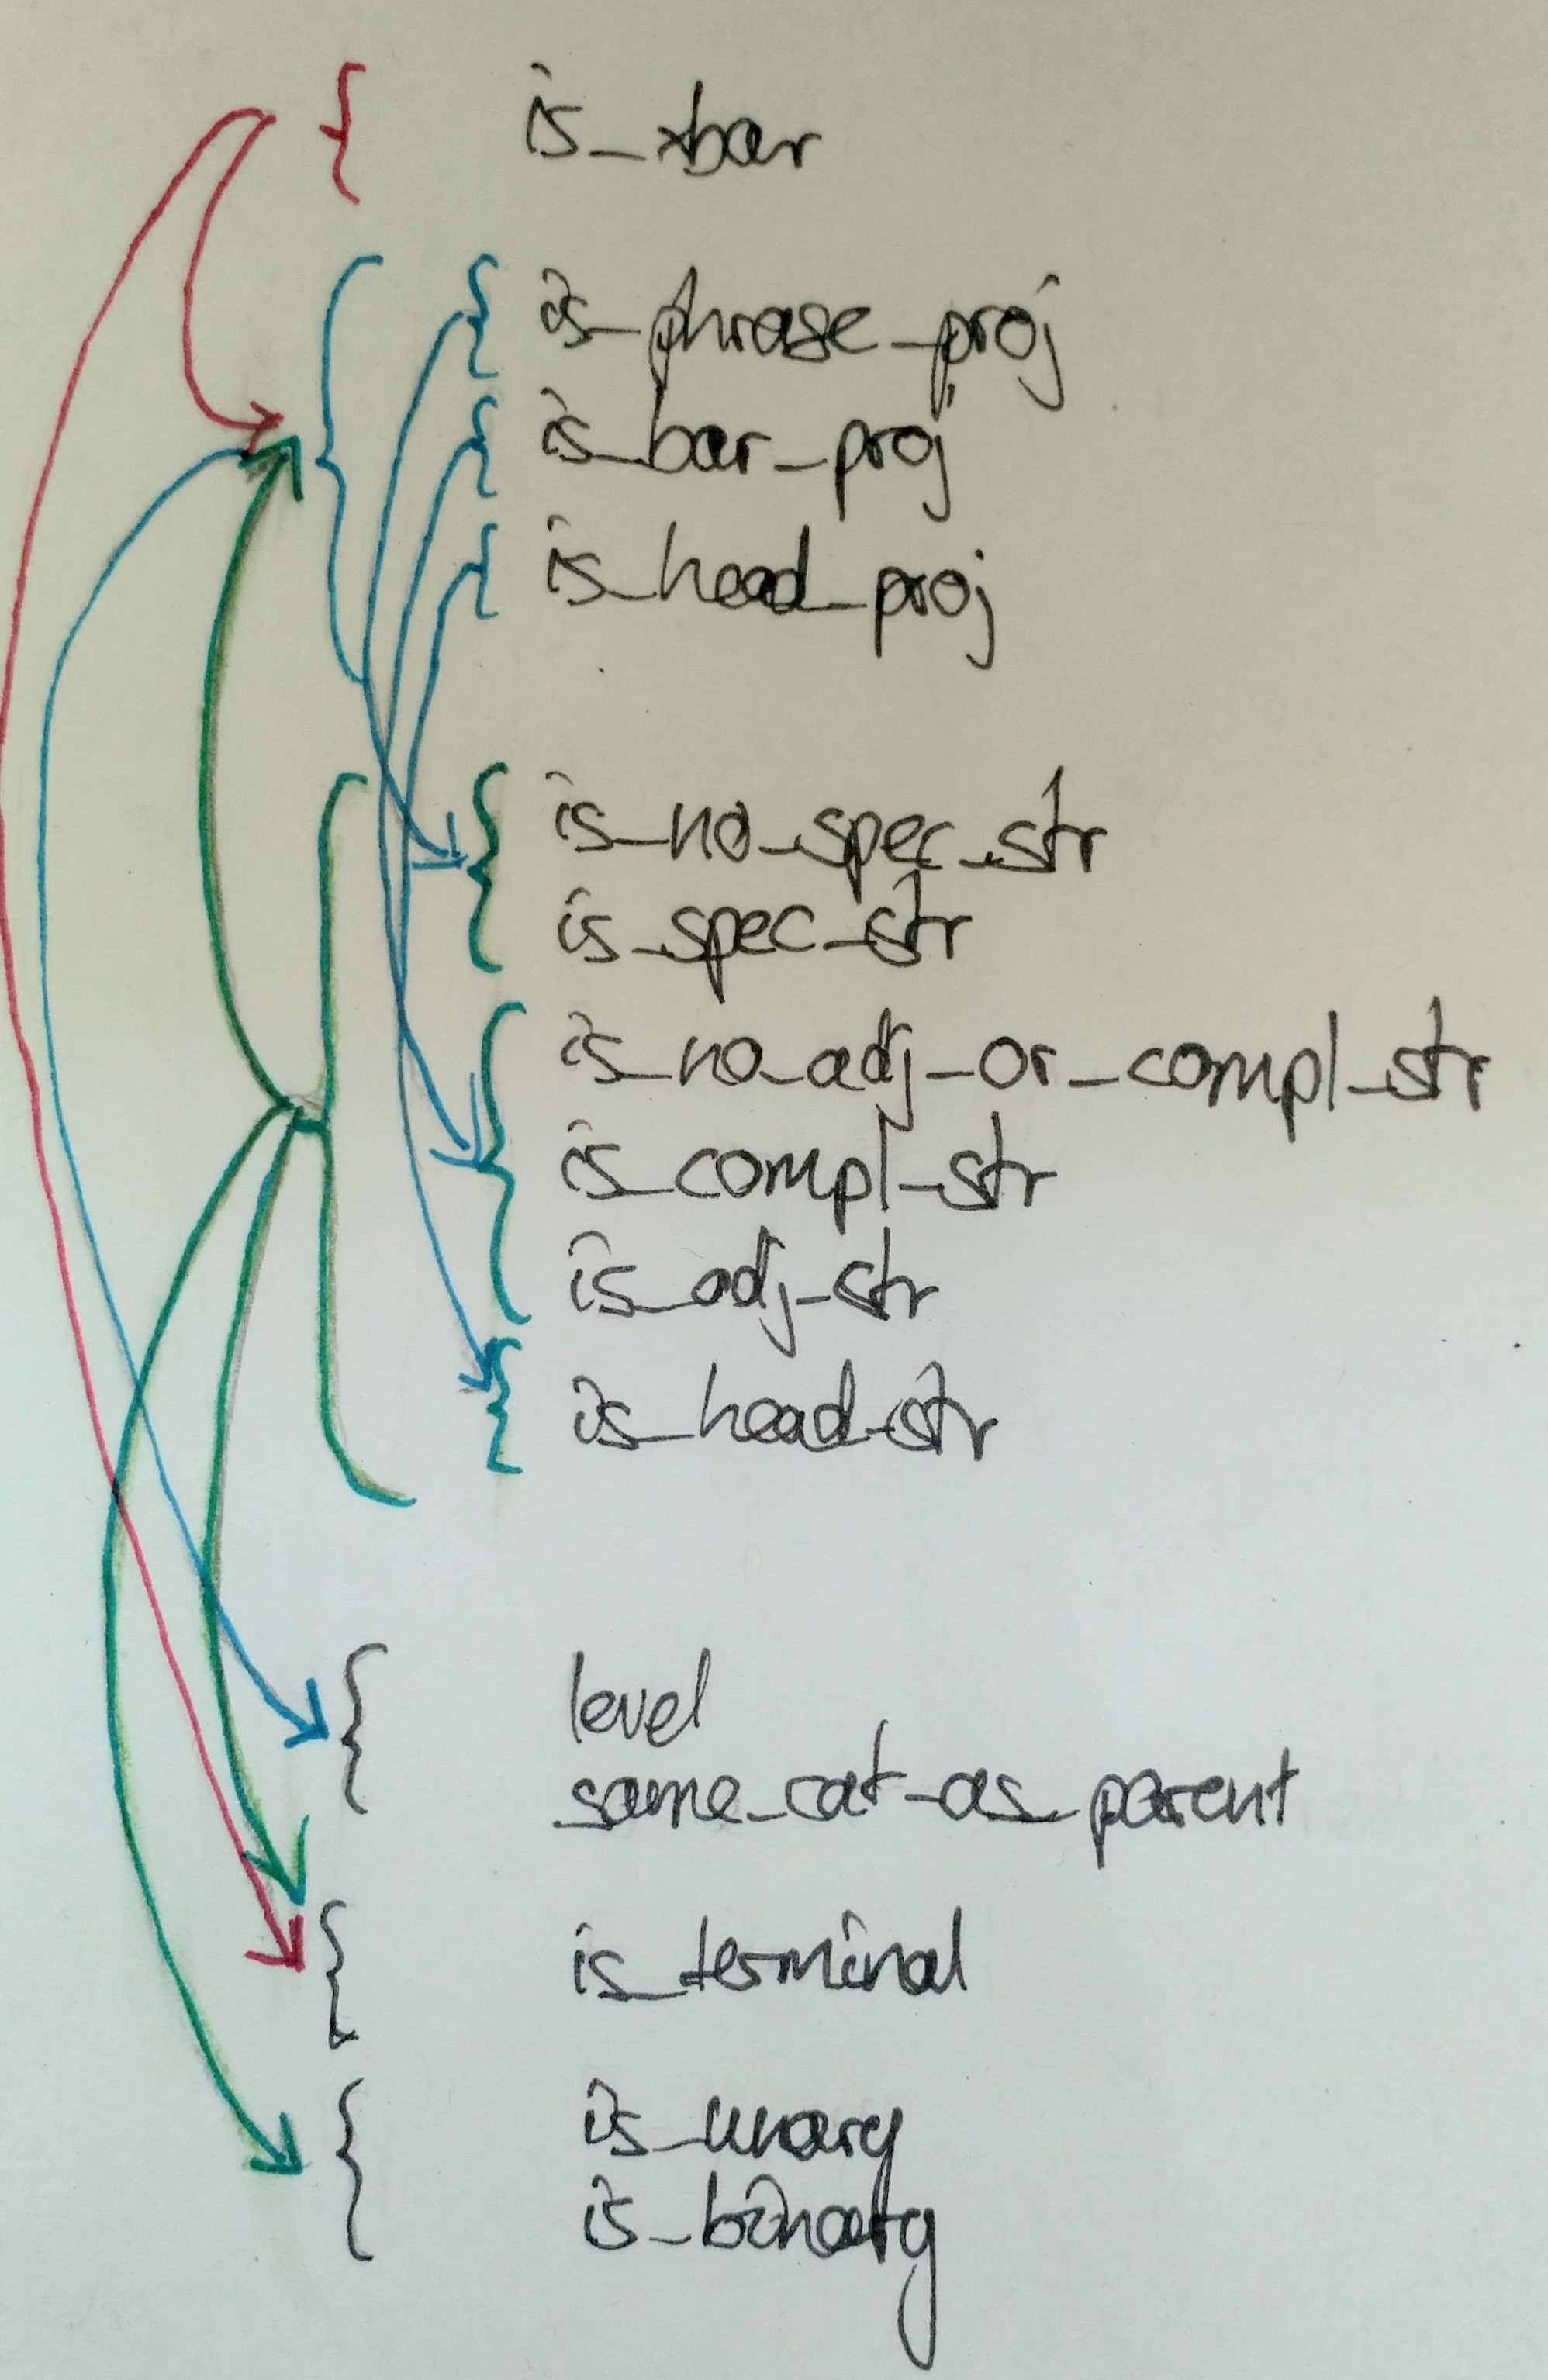
\includegraphics[width=8cm]{call_structure.jpg}\\
As you can see, there is no direct recursion (no function that calls itself in its definition); instead the cyclic structure enters through the projection functions (blue) calling the structure functions (green), which in turn call the projection functions again, thereby creating an indirect recursion.


\end{task}

\end{document}
